In order to generate a visualization of the light curve over time, the cleaned data was loaded into
a python script using the \texttt{pandas} library. The data was plotted using \texttt{matplotlib}, 
with Heliocentric Julian Date (HJD) values on the x-axis and relative flix on the y-axis.
We used Python-based strategies described by Scopatz and Huff \cite{scopatz2015effective} 
for automation and visualization.

The resulting plot, a light curve, shows how the brightness of the system changes over time. This 
shows a clear representation of the systems periodic behavior, while also showing the primary 
eclipse.

Figure~\ref{fig:lightcurve} shows the light curve of Target 1. A clear drop in brightness reveals 
the likely time of the primary eclipse. This figure serves as a oundation for the quantitative 
analysis.

\begin{figure}[h!]
	\centering 
	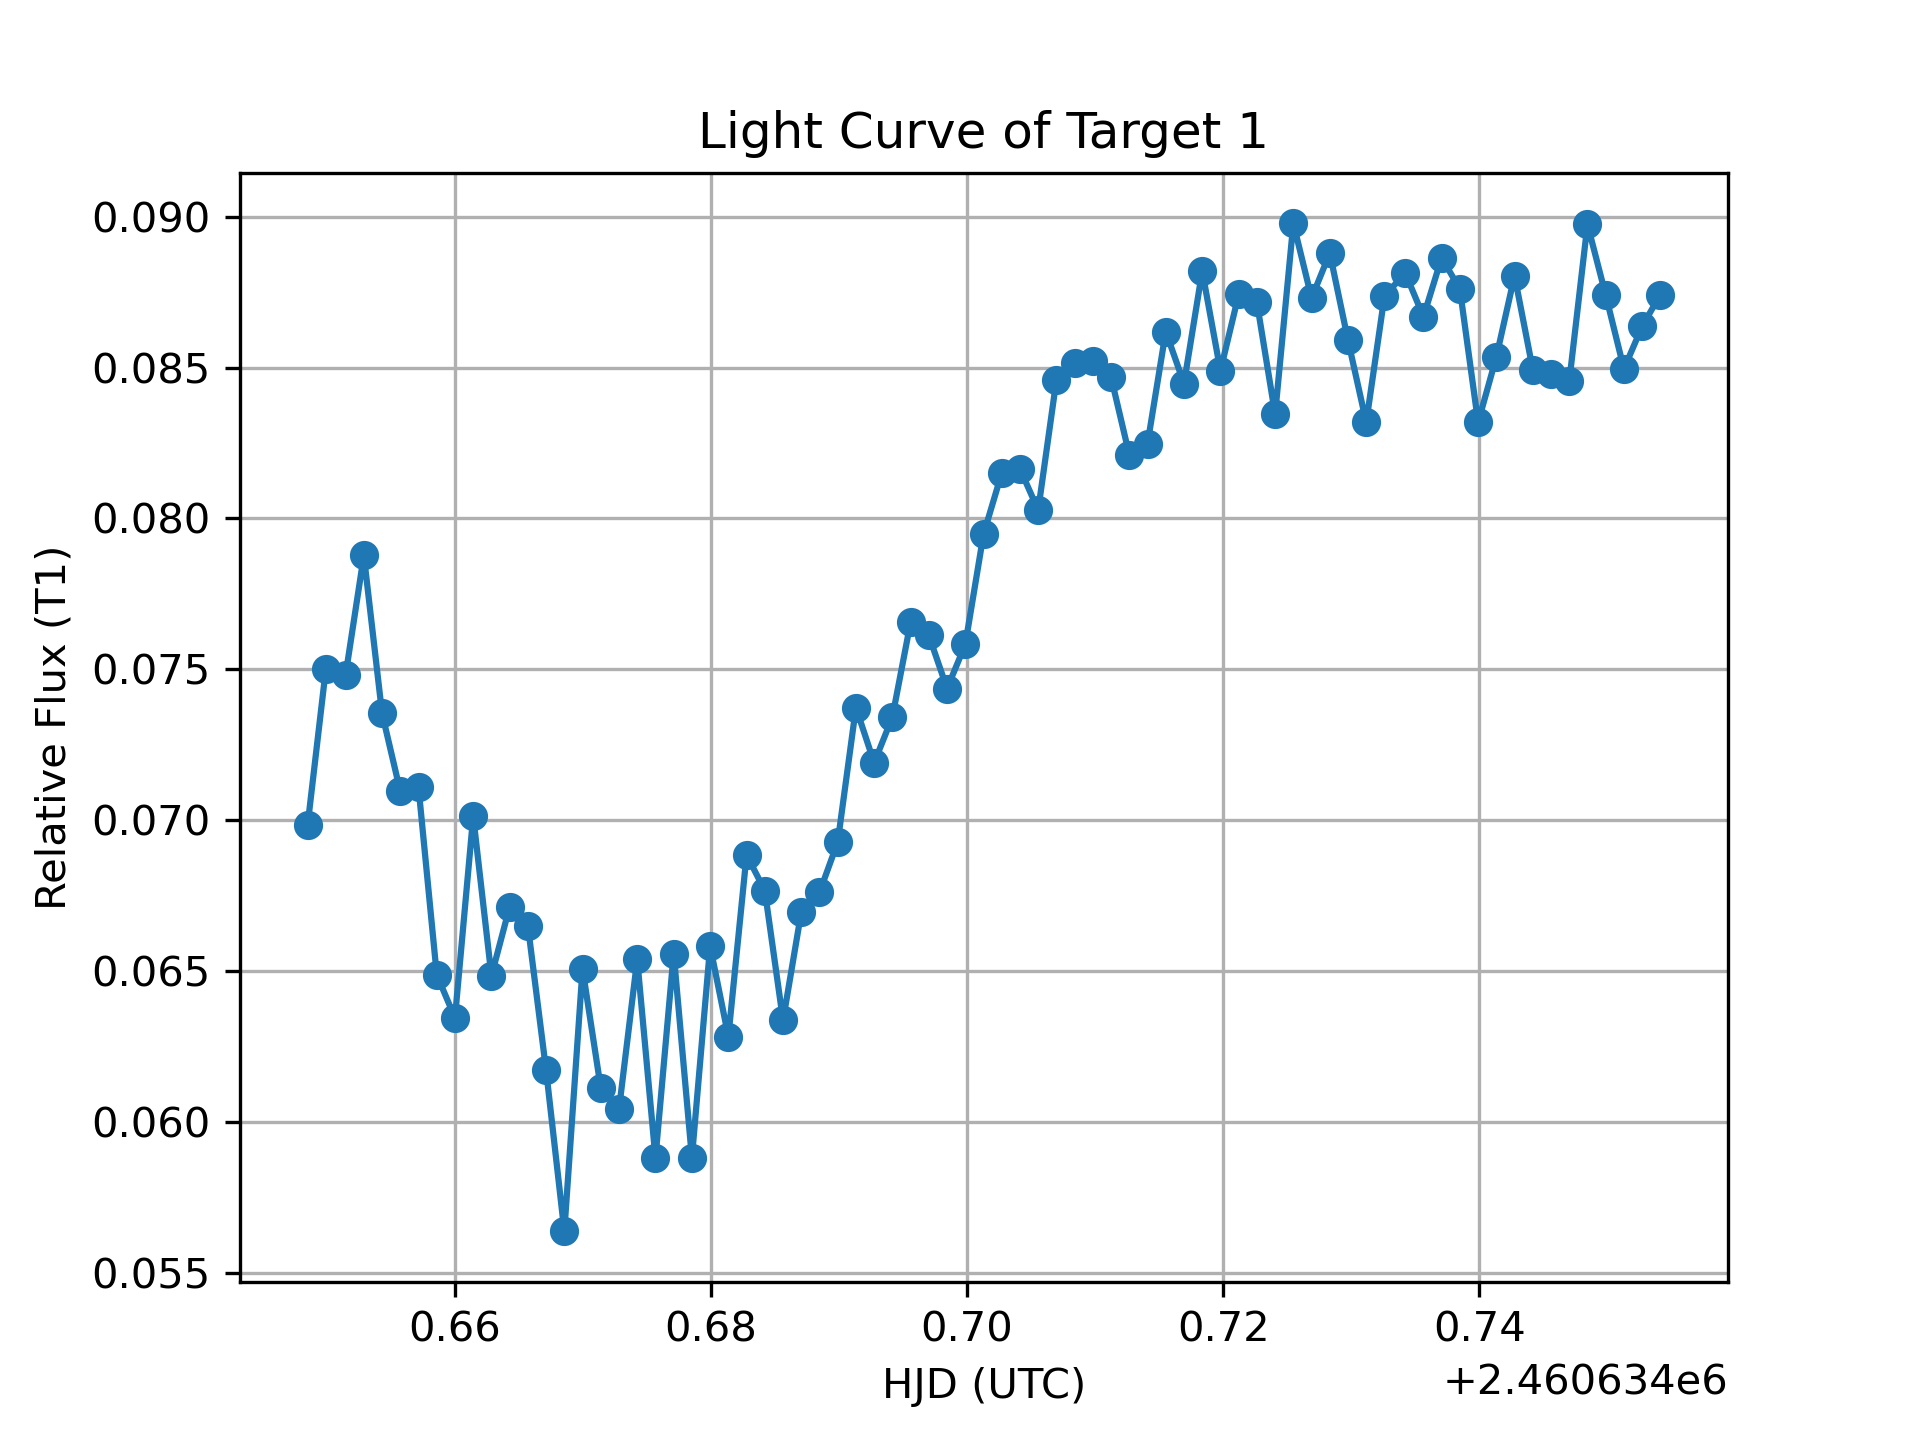
\includegraphics[width=0.8\textwidth]{figs/light_curve.png}
	\caption{Light curve of Target 1 plotted from telative flux measurments over time.}
	\label{fig:lightcurve}
\end{figure}
